\section{Fragment InicioSesion}
Aunque el nombre del insinúe que se se emplea para acceder a una cuenta de usuario, en realidad se trata de un fragmento que permite seleccionar entre una serie de facultades. El nombre se debe a que en el primer prototipo se implementó un inicio de sesión que fue finalmente sustituido, para evitar conflictos y complicaciones se decidió conservar el nombre pero no la funcionalidad original.

Mediante una lista de selección se nos pertmite situar nuestra ubicación predeterminada en una facultad específica. Además, la infomación adicional proporcionada por otros fragmentos, como los horarios de la biblioteca, muestran los de la facultad deseada. También existe la posibilidad de no elegir ninguna y mostrar información de la facultad más cercana.

\subsection{Variables}

\begin{itemize}
	\item indice$\_$facultad
	\item facultad$\_$spinner
	\item boton$\_$continuar
\end{itemize}

\textit{facultad$\_$spinner} es un spinner (lista de selección), mediante un ArrayAdapter le suministramos el string array (facultades) que hemos definido previamente con el nombre de las facultades, junto con la opción ninguna facultad seleccionada, que aparece al principio. Dicho string array está definido en el archivo string.xml.

La variable \textit{indice$\_$facultad} es una variable estática que empleamos para indicar al resto de fragmentos la facultad seleccionada. Cuando seleccionamos una facultad guardamos sus posición en la lista restando 1. Esto es debido a que las ubicaciones de las distintas facultades se almacenan en otra lista. Dicha lista no tiene la opcion ninguna facultad seleccionada. De forma que es necesario restar un 1 para que las posiciones se alineen.

La variable \textit{boton$\_$continuar} es un botón que al interactuar con él nos lleva al fragmento de página de inicio



\begin{figure}[H]
  \begin{subfigure}{0.5\textwidth}
    \centering
    % include first image
    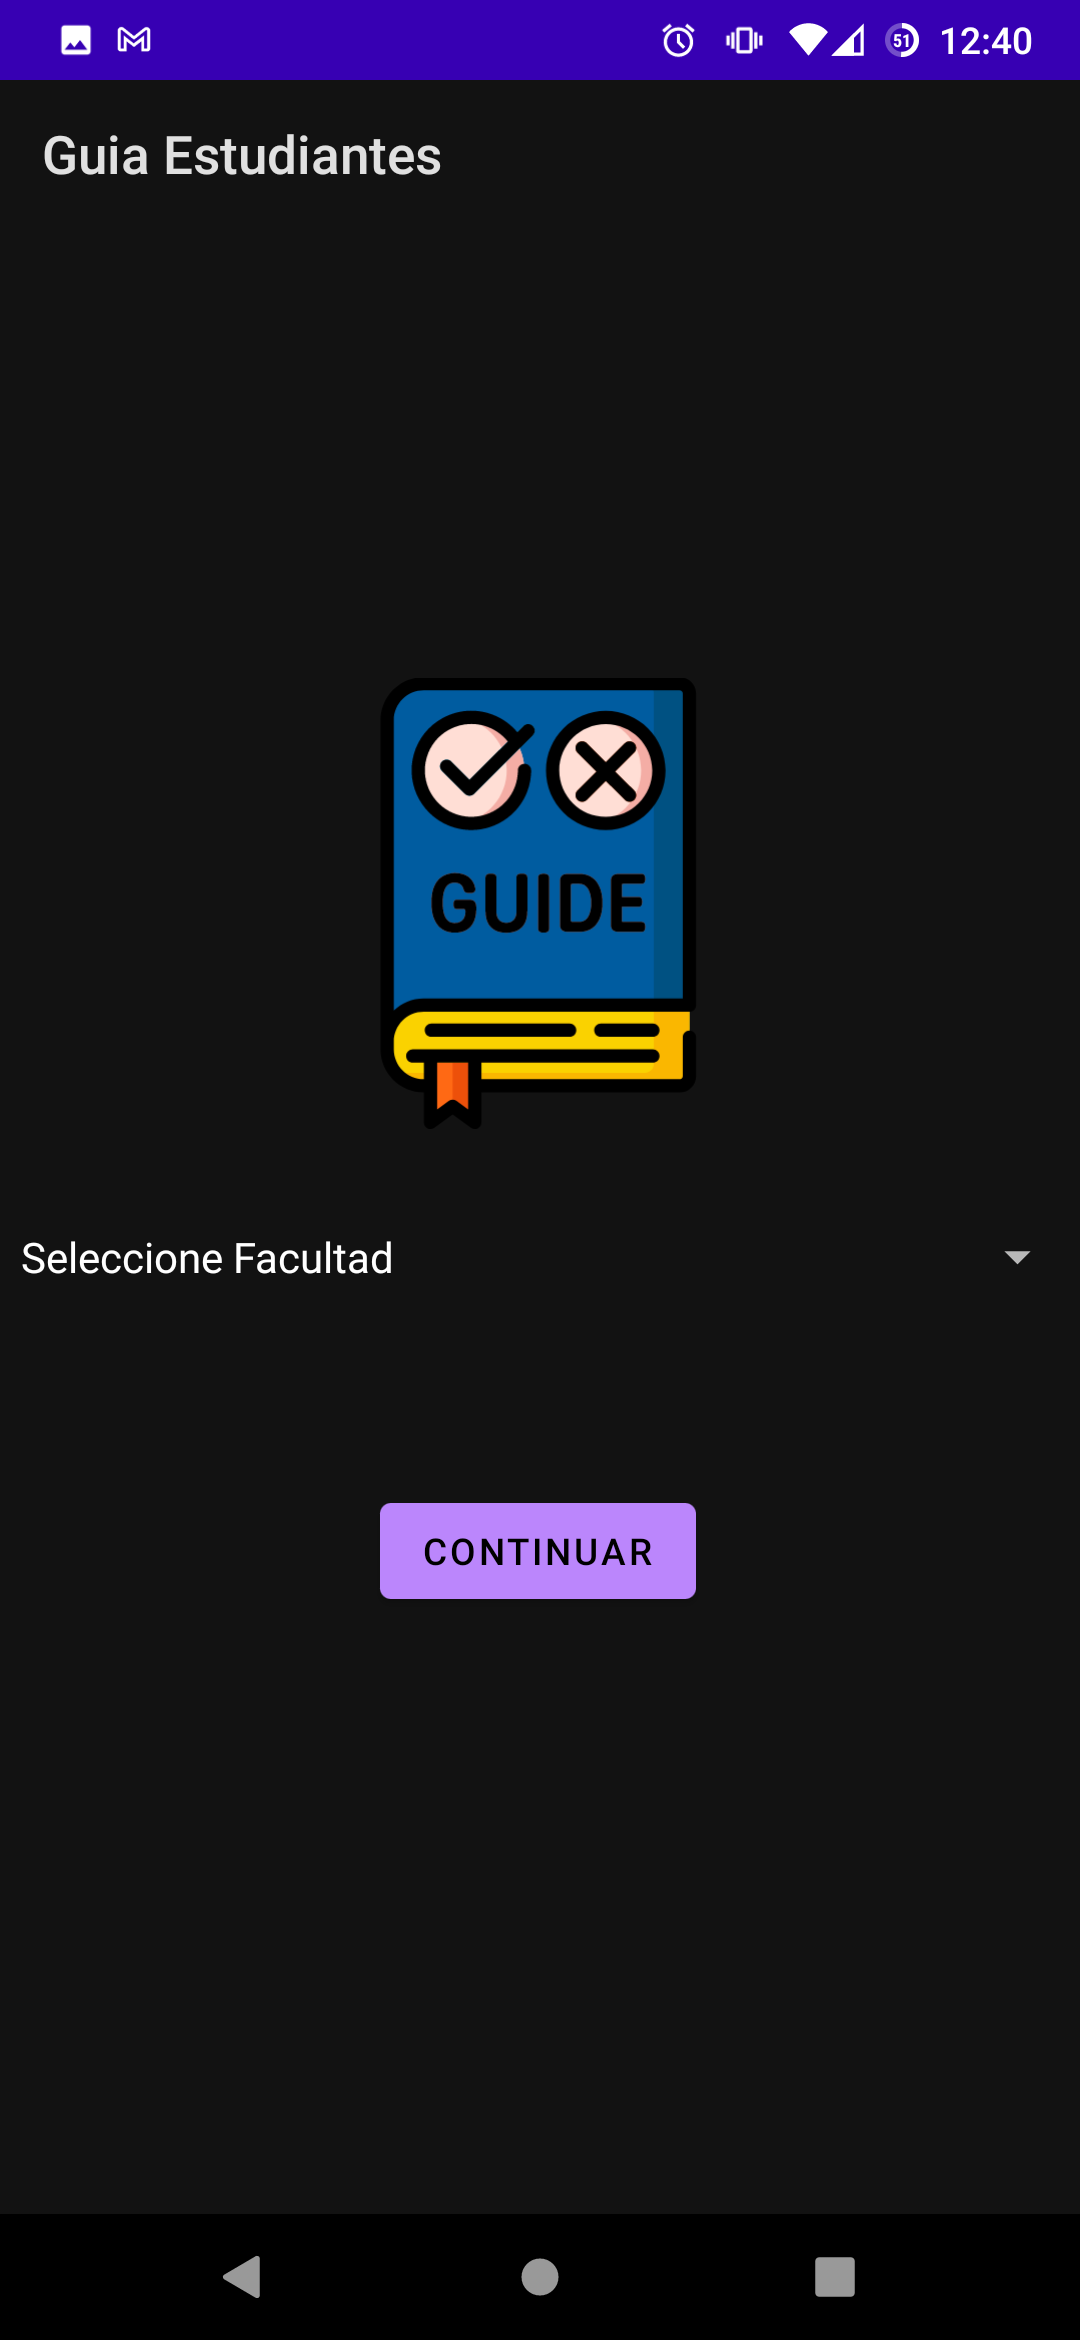
\includegraphics[width=1\linewidth]{inicio1.png}
    \caption{Página de inicio}
    \label{fig:sub-first}
  \end{subfigure}
  \begin{subfigure}{0.5\textwidth}
    \centering
    % include second image
	  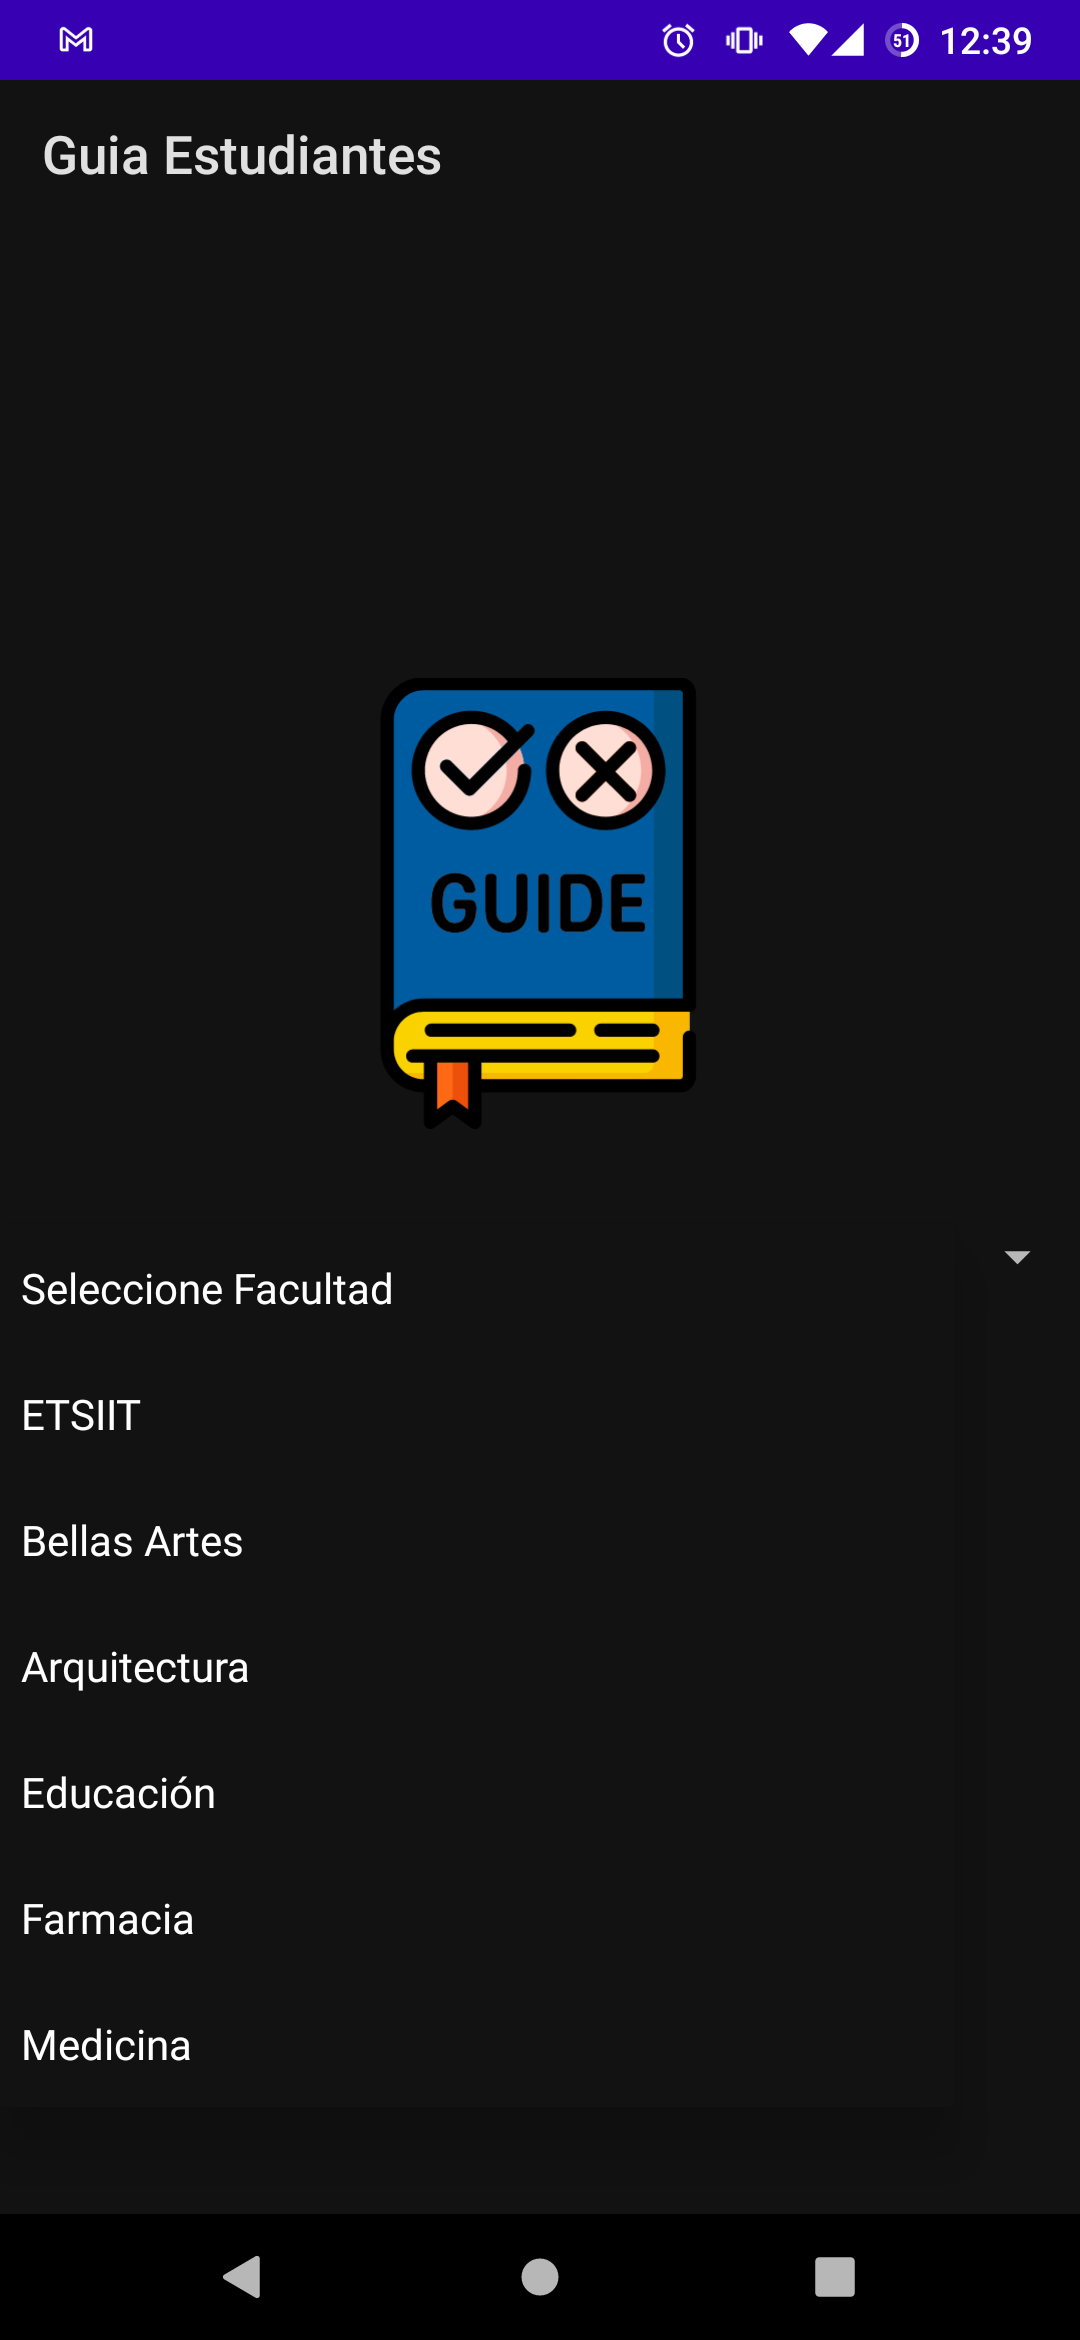
\includegraphics[width=1\linewidth]{inicio2.png}
    \caption{Página de inicio: Menú }
    \label{fig:sub-second}
  \end{subfigure}
\end{figure}



